\section{Theory}
All the terms utilized throughout this paper attain their meaning from the field of electrochemistry, unless specified otherwise. Furthermore, \textit{cathode} refers to the negative pole during process and the \textit{anode} refers to the positive pole during discharge.

\subsection{Sodium-Ion Batteries}
At their core, all modern batteries are based on a redox reaction. Through the exchange of electrons accompanying a sequence of oxidation and reduction, a charge can be stored and released\cite{Beerenwinkel2012}.
This is commonly facilitated through two electrodes capable of intercalating ions, separated by a separator and electrically connected through a conductive electrolyte. In the field of sodium-ion batteries (SIBs), layered-metal-oxide and a polyanionic anode are commonly paired with a hard-carbon cathode and a liquid carbonate ester electrolyte\cite{Xiang2015,Che2017,Xie2020}.
Solid electrolytes exist but are less common\cite{Dai2021}. Through the intercalation of sodium-ions in the hard-carbon during the charging process, a charge and thus a potential is built up between the two electrodes, which can be harnessed as electrical energy during discharge. Most commonly, the sodium-ions are transferred from the anode to the cathode upon charge and returned upon discharge.
The experiment performed during this investigation slightly alters this process and only exchanges the sodium-ions between the cathode and the electrolyte. In the discharged state, the sodium-ions are bound to perchlorate in the electrolyte solution and only intercalate in the TiO2 cathode upon the application of a current to the cathode through the charging process, as explained by Wu Liming et al\cite{Wu2015} and as visible in equation \ref{eq:sodiumintercalation}. This reduction requires the addition of electrons. Concurrently, the perchlorate-ions are intercalated in the graphite anode, as seen in equation \ref{eq:perchlorateintercalation}. This oxidation releases electrons. The charging process can thus be represented by the following reactions taking place at the two electrodes concurrently.

\begin{align}\label{eq:sodiumintercalation}
    \ce{TiO2 + NaClO4 + e- &-> NaTiO2 + ClO4- \\\label{eq:perchlorateintercalation}
    C6 + NaClO4 &-> C6 ClO4 + Na+ +e-}
\end{align}

During discharge, the reversed reactions occur at the same electrodes to facilitate a reversed current flow through an external circuit, where electrons would be taken up by the anode and released by the cathode. Thus, a complete reaction of the battery constructed is shown in eq. \ref{eq:fullbatteryeq}, with the charging process being visible from left to right and the discharge from right to left.

\begin{equation}\label{eq:fullbatteryeq}
    \ce{C6 + NaClO4 + TiO2 <=> C6 ClO4 + NaTiO2}
\end{equation}

\begin{figure}[ht]
    \centering
    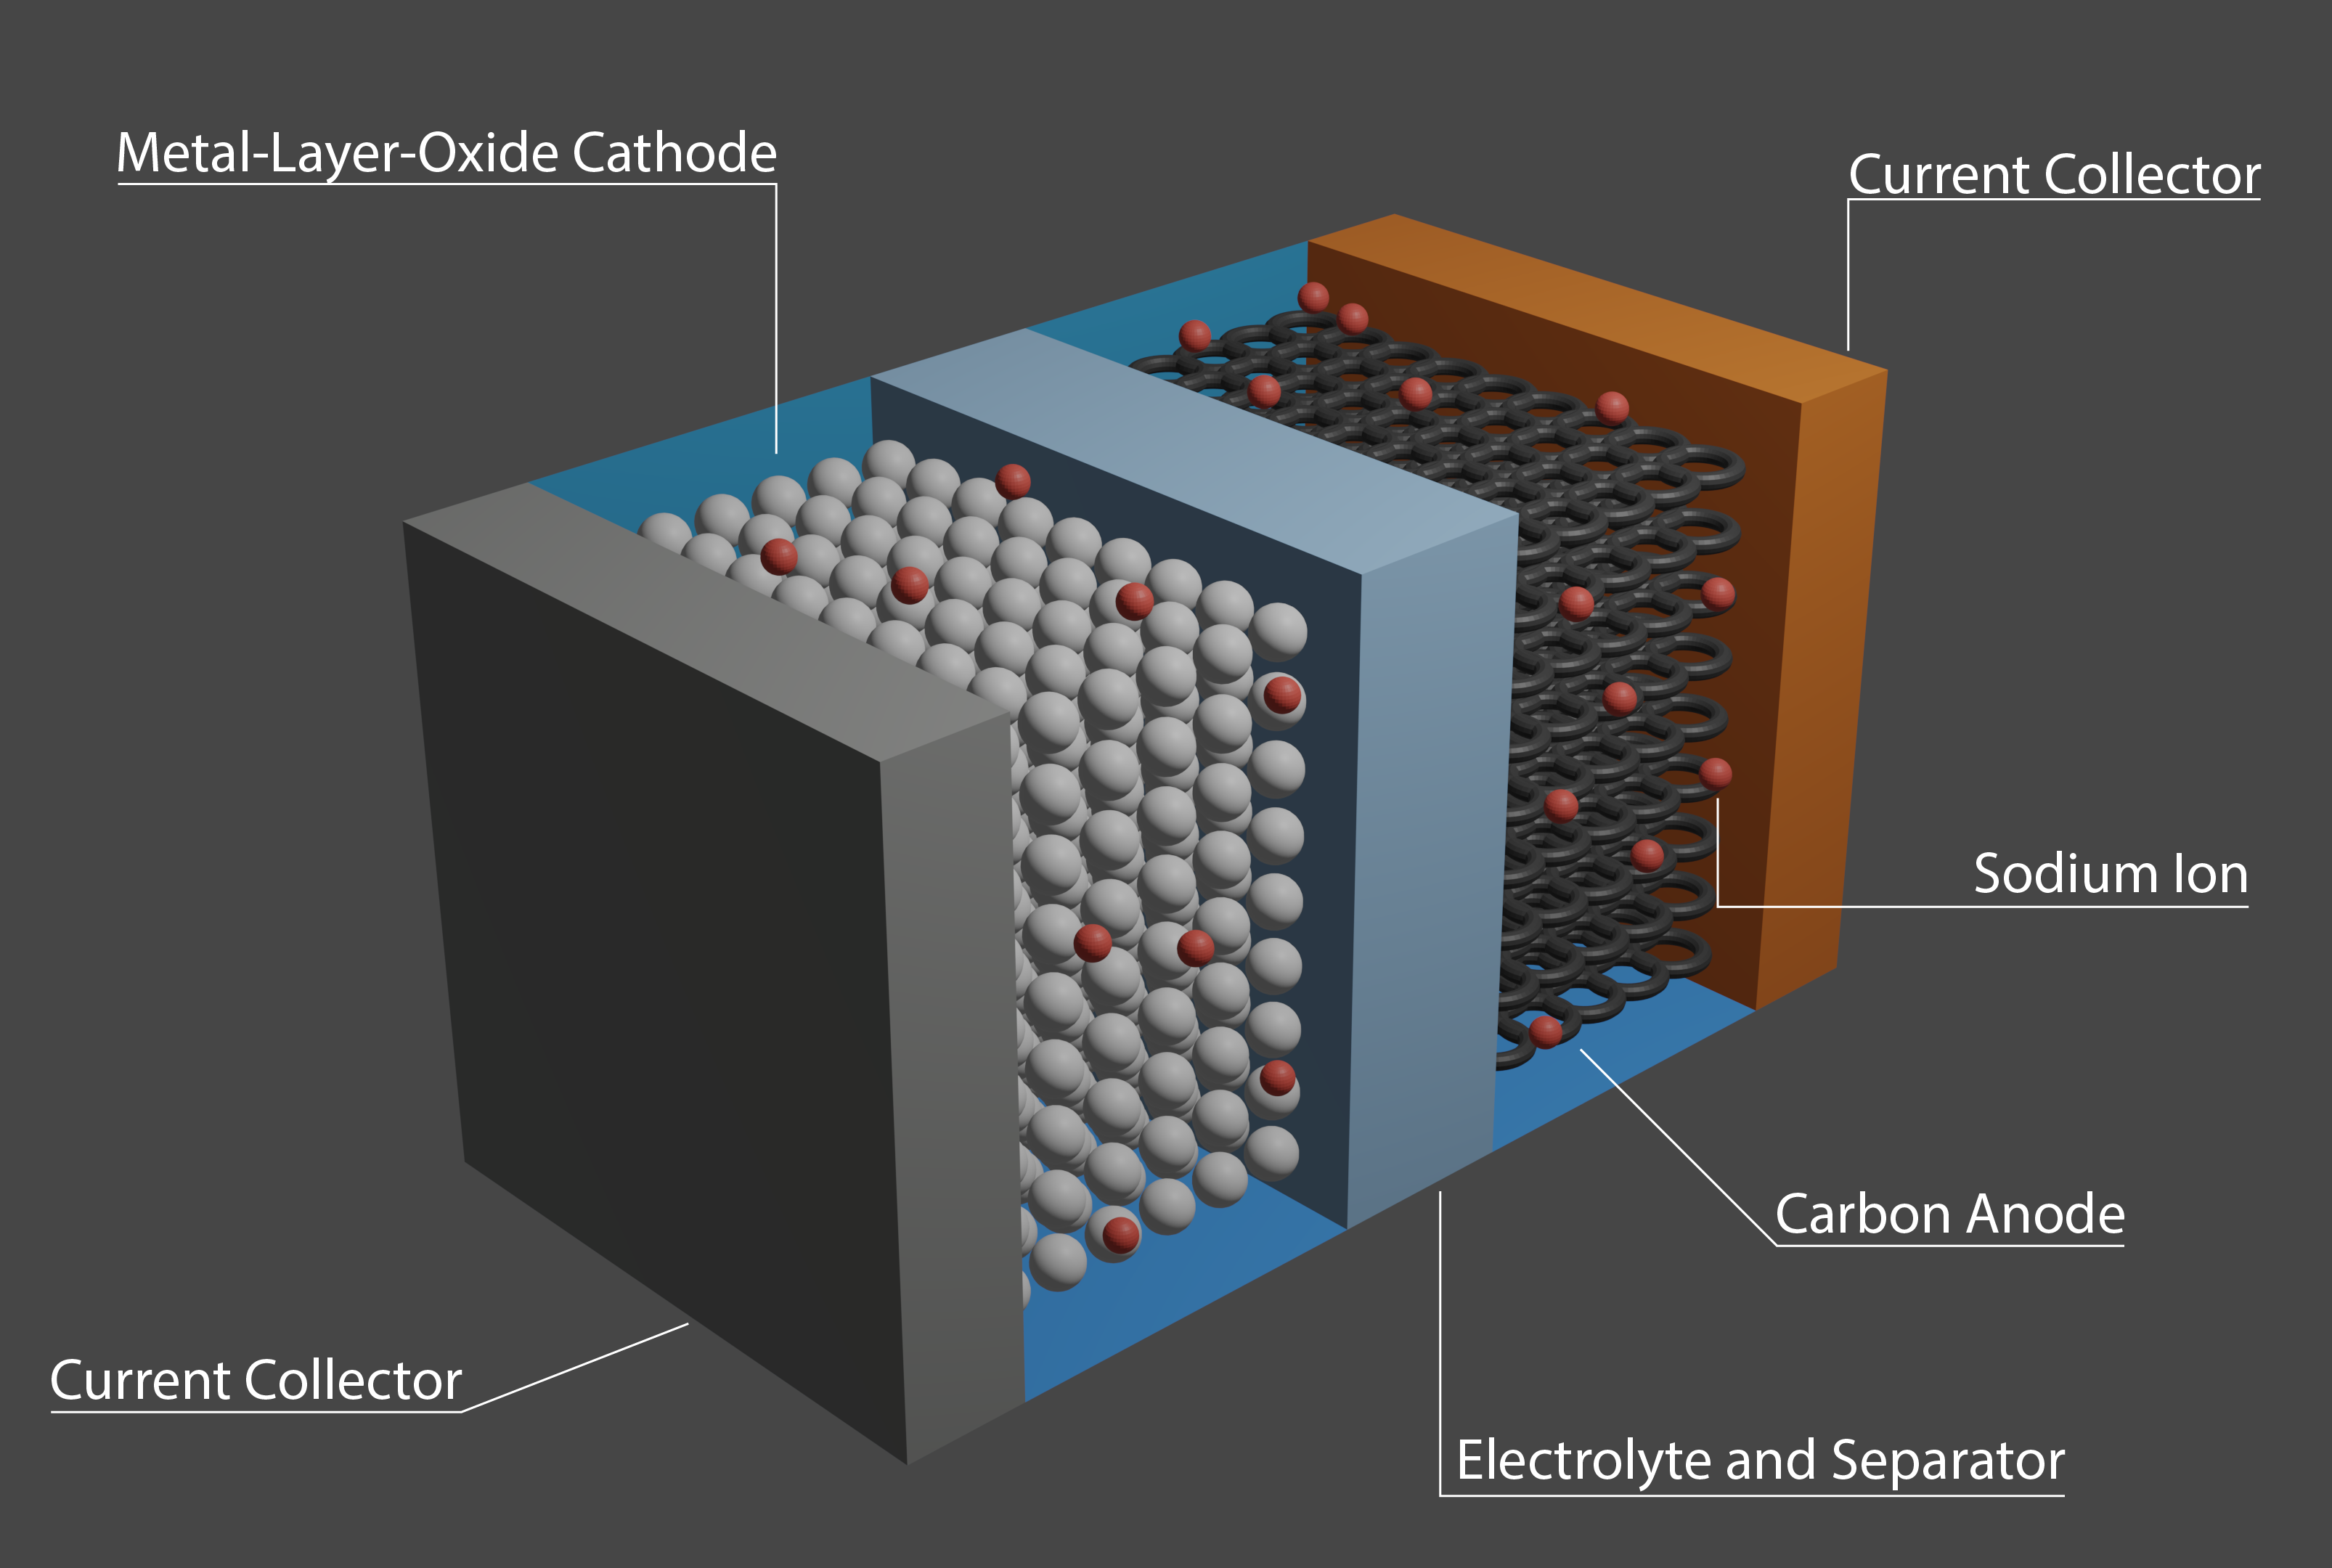
\includegraphics[width=\textwidth]{images/sodium_ion_battery_figure.png}
    \caption{A diagram depicting the basic layout of a sodium-ion battery.}
    \label{fig:sodiumbatterydiagram}
\end{figure}

\newpage

\subsection{Battery Evaluation}

To help compare and evaluate a battery, its capacity and power can be calculated. The capacity, also known as the charge, is based on total current flow, as visible in equation \ref{eq:capacityequation}:

\begin{equation}\label{eq:capacityequation}
    I = \frac{\Delta Q}{\Delta t} \Rightarrow \Delta Q = I \cdot \Delta t
\end{equation}
\begin{align*}
    Q &: \text{Capacity in coulombs [\unit{\C}]}\\
    I &: \text{Current in amperes [\unit{\A}]}\\
    t &: \text{time in seconds [\unit{\s}]}
\end{align*}

Similarly, the average power can be determined through the average current and average voltage, as seen in equation \ref{eq:powerequation}:

\begin{equation}\label{eq:powerequation}
    P = U \cdot I
\end{equation}
\begin{align*}
    P &: \text{Electric power in watt [\unit{\W}]}\\
    U &: \text{Voltage in [\unit{\V}]}
\end{align*}